\documentclass[onecolumn,notitlepage,letterpaper,aps,pra,12pt]{article}
\usepackage[utf8]{inputenc}
\usepackage[spanish, es-tabla]{babel}
\usepackage[T1]{fontenc}
\usepackage[version=3]{mhchem}
\usepackage{titlesec}
\usepackage{enumitem}
\usepackage{pdfpages}
\usepackage{setspace}  
\usepackage{lmodern}
\usepackage{beamerarticle}
%\usepackage{multicol}
\usepackage{fancyhdr}
\usepackage{graphics}
\usepackage{graphicx}
%\usepackage{natbib}
\usepackage[backend=bibtex,style=phys,natbib=true]{biblatex}

% Redefinimos el formato de los números en la bibliografía
\DeclareFieldFormat{labelnumberwidth}{[#1]} % Cambia superíndices a corchetes
\setlength{\biblabelsep}{0.5em} % Espacio entre el número y la referencia

\addbibresource{references.bib}
\DeclareFieldFormat[article]{title}{#1}
\usepackage{subfigure}
\usepackage{svg}
\usepackage{multirow} 
\usepackage{amssymb, amsmath, amsbsy} % simbolitos
\numberwithin{equation}{section}
\usepackage{upgreek} % para poner letras griegas sin cursiva
\usepackage{cancel} % para tachar
\usepackage{mathdots} % para el comando \iddots
\usepackage{mathrsfs} % para formato de letra
\usepackage{geometry}
\geometry{
	a4paper,
	total={150mm,257mm},
	left=20mm,
	top=20mm,
}
%\titleformat*{\section}{\bfseries\large}
%\titleformat*{\subsection}{\bfseries\normalsize}
\titleformat*{\section}{\normalfont\Large\bfseries\color{darkgray}}
\titleformat*{\subsection}{\normalfont\large\bfseries\color{gray}}
\titleformat*{\subsubsection}{\normalfont\normalsize\bfseries\color{blue}}
\usepackage{fancyhdr}
\pagestyle{fancy}
\rfoot{PROPUESTA DE INVESTIGACIÓN}
\renewcommand{\headrulewidth}{3pt}
\usepackage{tabularx}
\usepackage{supertabular}
\usepackage{vmargin}
\usepackage{mathtools} 
\usepackage{amsfonts}
\usepackage{float}
\usepackage{parskip}
\usepackage{times}
\usepackage{calligra}
\usepackage{latexsym}
\usepackage{booktabs}
\usepackage{tabulary}
\usepackage{caption}
\usepackage{url}
\spanishdecimal{.}
\usepackage{ragged2e}
%\bibliographystyle{unsrt}
\usepackage[usenames,dvipsnames]{pstricks}
\usepackage{epsfig}
\usepackage{pst-grad} % For gradients
\usepackage{pst-plot} % For axes
\usepackage{colortbl}
\usepackage{hyperref}
\usepackage{latexsym}
\usepackage{xcolor}
\usepackage{fancyhdr}
\usepackage{balance}
\usepackage{float}
\usepackage{bbold}
\usepackage[normalem]{ulem}
\usepackage{physics}
\usepackage{derivative}
\usepackage{tcolorbox}
\usepackage{amssymb}

% New commands
\newcommand{\miguel}[1]{{\color{magenta}#1}} 
\newcommand{\ricardo}[1]{{\color{red}#1}} 

%%%%%%%%%%%%%%%%%%%%%%%%%%%%%%
%%%%%%%%%%%%%%%%%%%%%%%%%%%%%%
\begin{document} 
%%%%%%%%%%%%%%%%%%%%%%%%%%%%%%
%%%%%%%%%%%%%%%%%%%%%%%%%%%%%%

\clearpage
\thispagestyle{empty}

%%%%%%%%%%%%%%%%%%%%%%%%%%%%%%
%%%%%%%%%%%%%%%%%%%%%%%%%%%%%%
\begin{titlepage}
\centering
\begin{figure}
    \centering
    
\includegraphics[width=4.5 in]{Images/uam.png}
\end{figure}

\vspace{1cm}

{\LARGE \rule{15cm}{1.0mm}  \par}

\centering
\vspace{0.45cm}

{\LARGE División de Ciencias Básicas e Ingeniería}

\centering
\vspace{0.45cm}

{\LARGE Posgrado en Ciencias (Física)}

\centering
\vspace{0.45cm}

{\LARGE Propuesta de Investigación Doctoral}

\vspace{0.25cm}

{\Huge \textbf{Fenómenos fuera de equilibrio en sistemas multimodo espín-bosón}}

\vspace{0.45cm}
{\large Propuesto por: {\bf M. en C. Ricardo Herrera Romero} \par}

\vspace{0.45cm}
{\large Matrícula: {\bf 2221801209} \par}

\vspace{0.45cm}
{\large Para sustentar el {\bf Examen Predoctoral} \par}

\vspace{0.45cm}
{\large Asesor: \textbf{Dr. Miguel Angel Bastarrachea Magnani}  \par}

\vspace{1cm}
\rule{5cm}{0.3mm}

\vspace{0.45cm}
{\large Coordinador: \textbf{Dr. Orlando Guzmán López}  \par}

{\LARGE \rule{15cm}{1.0mm}  \par}

\vspace{0.4cm}

{\large 18 de marzo de 2025 \par}
\vspace{0.1cm}
{\large Iztapalapa, Ciudad de México \par}
\end{titlepage}

%%%%%%%%%%%%%%%%%%%%%%%%%%%%%%
%%%%%%%%%%%%%%%%%%%%%%%%%%%%%%
\clearpage
\tableofcontents
\clearpage
\newpage
%%%%%%%%%%%%%%%%%%%%%%%%%%%%%%
%%%%%%%%%%%%%%%%%%%%%%%%%%%%%%

%%%%%%%%%%%%%%%%%%%%%%%%%%%%%%
%%%%%%%%%%%%%%%%%%%%%%%%%%%%%%
%\section*{Resumen}
%%%%%%%%%%%%%%%%%%%%%%%%%%%%%%
%%%%%%%%%%%%%%%%%%%%%%%%%%%%%%

%%%%%%%%%%%%%%%%%%%%%%%%%%%%%%
%%%%%%%%%%%%%%%%%%%%%%%%%%%%%%

%%%%%%%%%%%%%%%%%%%%%%%%%%%%%%
%%%%%%%%%%%%%%%%%%%%%%%%%%%%%%
\section{Introducción}
%%%%%%%%%%%%%%%%%%%%%%%%%%%%%%
%%%%%%%%%%%%%%%%%%%%%%%%%%%%%%

Hola 

En las últimas décadas, los sistemas de interacción spin-bosón se han convertido en un área central en la física~\cite{haroche2006} CITAR. El desarrollo de plataformas experimentales como cavidades y circuitos en electrodinámica cuántica (\textit{Quantum Electrodynamics} o QED)~\cite{Blais2021,Clerk2020}, sistemas de átomos fríos~\cite{Mekhov2012}, trampas ópticas~\cite{Yuanjie2021} o semiconductores acoplados a microcavidades~\cite{Schneider2018}, han permitido explorar el acoplamiento controlado entre excitaciones bosónicas (fotones) y sistemas discretos de dos niveles (qubits o átomos de espin $1/2$). %Más allá de su interés en óptica cuántica, estas arquitecturas  funcionan como simuladores cuánticos de fenómenos colectivos~\cite{caballero2016}.

Los sistemas abiertos y fuertemente acoplados, donde la interacción entre spin-bosón es comparable o mayor que las frecuencias propias del sistema— han cobrado relevancia experimental en los últimos años~\cite{Grifoni1999,ZhangHou2015,Burger2022,Fazio2025}. La disipación y el bombeo generan estados de equilibrio dinámico con coherencia colectiva, que reflejan nuevas formas de comportamiento organizado~\cite{Sieberer2016,Halati2020,Chelpanova2025}. El interés se centra, por tanto, en la competencia entre coherencia, interacción spin-bosón y disipación, lo que permite comprender y controlar el comportamiento colectivo en regímenes de acoplamiento intenso~\cite{subasi2012,FornDiaz2019,Kirton2019,LeBoite2020}.

Es en este marco conceptual modelos de spin-bosón como Rabi y Dicke adquieren relevancia, permitiendo analizar la dinámica de bombeo y disipación en estos sistemas [CITAR]. La propuesta de tesis doctoral se enmarca en esta dirección, con un enfoque sistemático y progresivo: comenzar con el modelo de Rabi abierto y avanzar hacia el modelo de Dicke abierto, incorporando tanto múltiples qubits como múltiples modos bosónicos, para explorar la interacción colectiva y multimodal en presencia de bombeo y disipación.




%%%%%%%%%%%%%%%%%%%%%%%%%%%%%%
%%%%%%%%%%%%%%%%%%%%%%%%%%%%%%
\subsection{Modelos de interacción espín-bosón}
%%%%%%%%%%%%%%%%%%%%%%%%%%%%%%
%%%%%%%%%%%%%%%%%%%%%%%%%%%%%%

El análisis de la interacción entre la radiación y un sistema de dos niveles (spín-bosón) tiene su origen en el modelo de Rabi, formulado para describir el acoplamiento coherente entre un solo átomo y un modo del campo electromagnético~\cite{rabi1936}. Su Hamiltoniano,

\begin{gather}
    \hat{H}_{\text{Rabi}} = \omega\hat{a}^{\dagger}\hat{a} + \frac{\omega_{0}}{2}\hat{\sigma}_{z} + g\left( \hat{\sigma}_{+} + \hat{\sigma}_{-} \right)\left( \hat{a}^{\dagger} + \hat{a} \right),
\end{gather}

describe la energía del campo (frecuencia $\omega$) y del átomo (frecuencia $\omega_{0}$) mediante los dos primeros términos, $g$ es el acomplamiento entre el campo y el átomo y $(\hat{\sigma}_{-}\hat{a} + \hat{\sigma}_{+}\hat{a}^{\dagger})$ conocido como termino ``rotante'' describe procesos que conservan el número total de excitaciones. Por ejemplo, $\hat{\sigma}_{+}\hat{a}$ corresponde a la emisión de un fotón $\hat{a}$ mientras el átomo se excita $\hat{\sigma}_{+}$ y viceversa con el término $\hat{\sigma}_{-}\hat{a}$. El modelo de Jaynes-Cummings~\cite{Jaynes1963}, se obtiene bajo la aproximación de onda rotante (RWA) que desprecia los términos $(\hat{\sigma}_{-}\hat{a} + \hat{\sigma}_{+}\hat{a}^{\dagger})$. Este término  ``contra-rotante'' no conserva el número de excitaciones: $\hat{\sigma}_{+}\hat{a}^{\dagger}$ crea simultaneamente una excitación atómica y un fotón, mientras $\hat{\sigma}_{-}\hat{a}$ aniquila ambas. La RWA es válida en el régimen de acoplamiento débil $(g<<\omega,\omega_{0})$. Bajo esta aproximación, el modelo de Jaynes-Cummings permite una solución exacta y estableció las bases de las cavidad QED al describir el intercambio coherente y periódico de una excitación~\cite{wallraff2004,Schoelkopf2008,devoret2013}.

Sin embargo, el progreso experimental ha permitido alcanzar regímenes de acoplamiento ultrastrong $(g/\omega \gtrsim 0.1)$ y deep strong $(g/\omega \gtrsim 1)$ donde la RWA deja de ser válida [Forn-Díaz et al., 2019; Yoshihara et al., 2017]. En estos regímenes, es necesario recurrir al modelo de Rabi completo, es decir, considerando los términos contra-rotantes.

La extensión natural del modelo de Rabi a sistemas con muchos átomos dio origen al modelo de Dicke~\cite{Dicke54}, que describe la interacción colectiva entre un conjunto de $N$ átomos idénticos y un único modo del campo electromagnético en una cavidad. El Hamiltoniano del modelo de Dicke se expresa como:
%%%
\begin{gather}
    \hat{H}_{\text{D}} = \omega\hat{a}^{\dagger}\hat{a} + \sum_{j=1}^{N}\left[ \frac{\omega_{0}}{2}\hat{\sigma}_{z}^{j} + \frac{g}{\sqrt{N}}\hat{\sigma}_{x}^{j}\left(\hat{a}^{\dagger} + \hat{a}\right) \right].
\end{gather}
%%%
Los primeros dos términos representan la energía del sistema en ausencia del acoplamiento luz-materia, $\omega$ es la frecuencia de un solo modo electromagnético confinado en la cavidad óptica, $\hat{a}^{\dagger}(\hat{a})$ es el operador de creación (aniquilación), $\omega_{0}$ es la frecuencia caracteristica individual de los átomos, $\hat{\sigma}_{z}^{j}$ es la matriz de espín de Pauli  y representa la diferencia de población entre el estado base y excitado de cada átomo individual. El tercer término incluye la interacción luz-materia donde $g$ es el acoplamiento entre los átomos y los fotones,  $N$ es el número de partículas y $\hat{\sigma}_{x}^{j}$ es una matriz de Pauli que representa el acoplamiento entre los dos niveles. 

Es posible aplicar la aproximación de onda larga~\cite{Dicke54}, la cual consiste en asumir que la longitud de onda del campo electromagnético  sea lo suficientemente grande como para que todos los átomos interactúen de la misma manera con él, comportándose colectivamente. Esta aproximación permite introducir los operadores de pseudospín colectivos  $\hat{J}_{\mu} = \frac{1}{2}\sum_{i=1}^{N}\hat{\sigma}_{\mu}^{i}$ (que siguen el álgebra SU(2)),  e incorporan el comportamiento colectivo del conjunto de átomos. Bajo esta consideración, el Hamiltoniano de Dicke se expresa de la siguiente forma: 
\begin{gather}\label{Dicke colectivo}
    \hat{H}_{\text{D}} = \omega\hat{a}^{\dagger}\hat{a} + \omega_{0}\hat{J}_{z} + \frac{2g}{\sqrt{N}}\hat{J}_{x}\left( \hat{a}^{\dagger} + \hat{a} \right).
\end{gather}


El interés en este modelo  radica en que predice fenómenos críticos como transiciones de fase cuánticas (\textit{Quantum Phase Transition} o QPT), donde el sistema exhibe un cambio abrupto en las propiedades del estado base al variar los parámetros como el acoplamiento luz-materia y transiciones de fase cuántica de estados excitados (\textit{Excited State Quantum Phase Transitions} o ESQPT)~\cite{Hepp73,wang1973,hioe1973,Sachdev99,Larson17}. 





Cuando la interacción luz-materia alcanza un valor crítico, el sistema experimenta una transición desde un estado normal, caracterizado por la ausencia de fotones, hacia un estado superradiante. %En este último, el número de fotones y átomos excitados se vuelve comparable al número total de átomos en el sistema. 
En este régimen, la emisión promedio de fotones es diferente de cero, manifestándose como una emisión coherente y colectiva, fenómeno conocido como superradiancia~\cite{gross1982}. El modelo de Dicke ha tenido una gran recepción en el ámbito de la información cuántica~\cite{Garraway2011,Kirton2019,LeBoite2020}, pues en los últimos años, se ha implementado experimentalmente en diversas plataformas como qubits superconductores~\cite{Blais04,Casanova10} y transiciones Raman asistidas por cavidades~\cite{Baden14,Nagy10} por mencionar algunos. 
%%%
\begin{figure}[H]
    \centering
    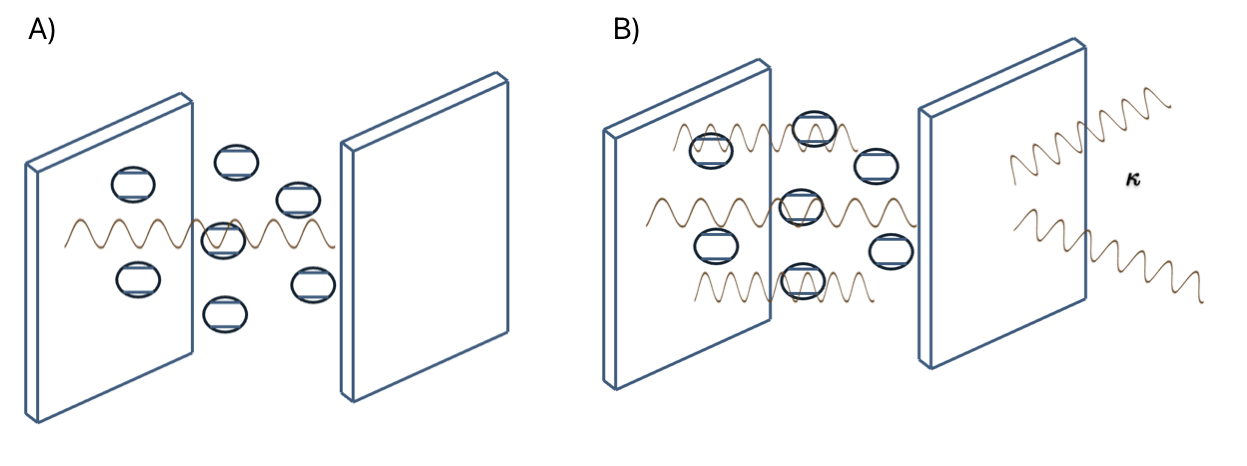
\includegraphics[width=0.9
\linewidth]{Images/cavity1.png}
    \caption{Ilustración del modelo de Dicke. 
A) Un conjunto de \( N \) átomos de dos niveles interactúa con un único modo de radiación electromagnética. 
B) Un conjunto de \( N \) átomos de dos niveles interactúa con múltiples modos de radiación electromagnética, incorporando además efectos de bombeo y disipación \( \kappa \).}
    \label{Figure Cavity}
\end{figure}

En el estudio del modelo de Dicke, la inclusión de interacciones entre los átomos permite explorar nuevos fenómenos críticos y modificaciones en la transición superradiante. En mi trabajo de maestría, investigué un modelo de Dicke anisotrópico que incorpora interacciones colectivas entre los emisores, analizando su diagrama de fases y la aparición de QPT y ESQPT. Utilizando técnicas semiclásicas, caractericé las superficies de energía y las densidades de estados, demostrando cómo estas interacciones pueden inducir nuevas fases y modificar los puntos críticos del sistema~\cite{Herrera2022}. Posteriormente, extendí este análisis, identificando modos de fase y amplitud, lo que proporciona una nueva perspectiva sobre la relación entre anisotropía y criticidad en sistemas luz-materia fuertemente acoplados~\cite{herrera2024}. El Hamiltoniano de Dicke anisotrópico con interacciones materiales es:
%%%
\begin{gather}
    \hat{H}_{\text{I}} = \omega\hat{a}^{\dagger}\hat{a} + \omega_{0}\hat{J}_{z} + \frac{\gamma}{\sqrt{N}}\left[ \hat{a}\hat{J}_{+} + \hat{a}^{\dagger}\hat{J}_{-} + \xi\left( \hat{a}\hat{J}_{-} + \hat{a}^{\dagger}\hat{J}_{+} \right)  \right] + \frac{1}{N}\sum_{i=x,y,z} \eta_{i}\hat{J}_{i}^{2}.
\end{gather}
%%%
Los términos $\hat{a}\hat{J}_{+}$ y $\hat{a}^{\dagger}\hat{J}_{-}$ son los rotantes, mientras que $\hat{a}\hat{J}_{-}$ y $\hat{a}^{\dagger}\hat{J}_{+}$ los contra-rotantes. El parámetro $\xi$, conocido como término anisotrópico, modula la no conservación del número de excitaciones. Los parámetros $\eta_{i}$ representan la intensidad de la interacción colectiva entre los emisores.


El Modelo de Dicke se ha estudiado extensamente considerando un solo modo $\omega$. %Al aplicar la aproximación de onda larga, es posible observar fenómenos críticos, como las transiciones de fase superradiantes colectivas, mencionadas previamente. 
Sin embargo, en los últimos años, ha surgido un creciente interés en explorar sistemas más complejos, como cavidades multimodo o redes de cavidades ópticas acopladas~\cite{tolkunov2007,fiorelli2020,carollo2021}, los cuales ofrecen una descripción más realista de la interacción spín-bosón. En estos sistemas, múltiples modos del campo electromagnético interactúan con los átomos de la cavidad. El Hamiltoniano de Dicke multimodo se expresa de la siguiente forma:
\begin{gather}
        \hat{H}_{\text{Multimodo}} = \sum_{k}\left(\omega_{k}\hat{a}^{\dagger}_{k}\hat{a}_{k} + \sum_{j=1}^{N}\left[ \frac{\omega_{0}}{2}\hat{\sigma}_{z}^{j} + \sum_{k}\frac{g_{k}}{\sqrt{N}}\hat{\sigma}_{x}^{j}\left(\hat{a}^{\dagger}_{k} + \hat{a}_{k}\right) \right]\right).
\end{gather}
Donde $\omega_{k}$ es la frecuencia de cada modo electromagnético. Esta extensión no solo enriquece el modelo teórico, sino que también permite explorar nuevos fenómenos físicos. Entre ellos destacan la competencia entre modos en las transiciones de fase cuánticas~\cite{tolkunov2007}, la formación de estructuras análogas a los vidrios de espín~\cite{rotondo2015}, la aparición de transiciones de fase no convencionales~\cite{kipf2014} y la manifestación de desorden en el sistema~\cite{vojta2013,das2024}. Estas propiedades no son solo de interés fundamental; tienen implicaciones prácticas directas, como demostró el experimento de Brendan P. Marsch, et al.~\cite{marsch2021}, donde un modelo de Dicke multimodo con un condensado de Bose-Einstein en una cavidad óptica se utilizó para almacenar múltiples patrones, un paso crucial hacia el desarrollo de memorias cuánticas y redes neuronales cuánticas~\cite{fiorelli2020}.




%Entender estos sistemas también tiene implicaciones prácticas como el diseño de memorias cuánticas~\cite{fiorelli2020}.  En el 2021, Brendan P. Marsh, et al.~\cite{marsch2021}, realizó un experimento basado en el modelo de Dicke multimodo utilizando condensados de Bose-Einstein y diferentes modos de radiación electromagnética en una cavidad óptica. %En el experimento, los átomos se colocan en una cavidad confocal, donde los modos de luz están degenerados, lo que permite una interacción colectiva entre los átomos y los fotones. 
%Esta configuración permite almacenar múltiples patrones de memoria en la red de espines, que pueden ser recuperados mediante la dinámica de relajación del sistema. %Este trabajo es relevante hacia la realización de redes neuronales cuánticas que combinen la potencia de la computación clásica con las ventajas de los efectos cuánticos. 

De forma paralela, la exploración de sistemas con múltiples átomos ha llevado al estudio de configuraciones novedosas como los ``átomos gigantes'', donde un solo átomo se acopla a un campo en múltiples puntos espaciales, introduciendo efectos no-Markovianos como retardos e interferencias [Kockum et al., 2018]. En conjunto, estas plataformas experimentales están verificando directamente las predicciones de los modelos extendidos de Dicke, haciendo urgente el desarrollo de marcos teóricos que integren de manera coherente la disipación, la multifrecuencia y las interacciones colectivas, objetivo central de esta tesis doctoral.


%%%%%%%%%%%%%%%%%%%%%%%%%%%%%%
%%%%%%%%%%%%%%%%%%%%%%%%%%%%%%
\subsection{Sistemas abiertos y dinámica fuera del equilibrio}
%%%%%%%%%%%%%%%%%%%%%%%%%%%%%%
%%%%%%%%%%%%%%%%%%%%%%%%%%%%%%

Por otro lado, la física de los sistemas cuánticos abiertos y fuera del equilibrio ha adquirido una relevancia creciente en las últimas décadas, al ofrecer un marco para describir fenómenos en una amplia variedad de plataformas, que van desde átomos fríos y condensados de Bose–Einstein hasta sistemas de materia condensada y óptica cuántica~\cite{rotter2015}.
A diferencia de los sistemas cerrados, cuya evolución temporal está gobernada únicamente por un Hamiltoniano conservativo, los sistemas abiertos interactúan  con su entorno, lo que introduce mecanismos de disipación, ruido y pérdida de coherencia~\cite{Sieberer2016}. Esta interacción con el medio externo altera la dinámica del sistema, dando lugar a estados estacionarios que no pueden describirse mediante estados puros, sino mediante por operadores de densidad~\cite{breuer2003}.

En este contexto, la energía puede tanto disiparse como inyectarse en el sistema. El bombeo coherente posibilita una transferencia de energía controlada que preserva la coherencia cuántica, mientras que el bombeo incoherente, de origen térmico o aleatorio, introduce ruido y pérdida de información. Así, los sistemas abiertos permiten estudiar cómo la coherencia y la disipación coexisten, se equilibran o incluso cooperan para dar lugar a dinámicas estacionarias fuera del equilibrio.

La evolución de este tipo de sistemas se describe a través de ecuaciones maestras para el operador de densidad. En particular, la ecuación de Lindblad proporciona un marco  para incorporar procesos de disipación y bombeo~\cite{Fazio2025} (Cita[Breuer y Petruccione, 2002]). A diferencia de los sistemas cerrados, los estados estacionarios obtenidos de esta descripción no corresponden a estados térmicos, sino a configuraciones mantenidas por flujos continuos de energía y partículas entre el sistema y su entorno.

De forma complementaria, el formalismo de Keldysh ofrece una poderosa formulación de campo fuera del equilibrio que permite tratar, de manera unificada, la coherencia y la disipación dentro de un mismo marco de acción efectiva~\cite{Fazio2025} (Cita[Sieberer et al., 2016]; Cita[Kirton et al., 2019]). Estas herramientas teóricas se han consolidado para describir la competencia entre coherencia, interacción y pérdida en las plataformas experimentales contemporáneas, como cavidades ópticas, circuitos superconductores y redes fotónicas (Cita[Blais et al., 2021]).

Las plataformas experimentales actuales —circuit QED, cavidades ópticas y iones atrapados— permiten manipular y medir con alta precisión la coherencia y el entrelazamiento, lo que ha impulsado aplicaciones directas en información cuántica, metrología y simulación (Cita[Ritsch et al., 2013]; Cita[Blais et al., 2021]). La posibilidad de controlar la disipación permite estabilizar estados entrelazados robustos o generar correlaciones persistentes mediante ingeniería del entorno (Cita[Diehl et al., 2008]). Además, los sistemas fuera del equilibrio ofrecen rutas para explorar fenómenos sin análogo en equilibrio, como condensados fotónicos o fases topológicas disipativas (Cita[Mivehvar et al., 2021]). 

%%%%%%%%%%%%%%%%%%%%%%%%%%%%%%
%%%%%%%%%%%%%%%%%%%%%%%%%%%%%%
\subsection{Modelo de Rabi y Dicke abierto}
%%%%%%%%%%%%%%%%%%%%%%%%%%%%%%
%%%%%%%%%%%%%%%%%%%%%%%%%%%%%%

Los modelos de Rabi y Dicke permiten estudiar la dinámica de sistemas abiertos y con disipación~CITAR. En el modelo de Rabi, en este contexto, emerge la transición de fase disipativa de segundo orden, donde el sistema alcanza un estado estacionario con un incremento significativo de excitaciones debido a la competencia entre el acoplamiento ultrastrong y la disipación HWANg. Aunque el número de excitaciones crece, el sistema sigue siendo finito, lo que permite observar esta transición de manera controlada incluso en sistemas pequeños.

El modelo de Dicke abierto y fuera de equilibrio describe la interacción luz–materia incorporando disipación (pérdida de fotones y relajación atómica) y un bombeo externo (emisión de láser). El bombeo y la disipación también dan lugar a transiciones de fase de carácter dinámico~\cite{kirton2017,LeBoite2020} como oscilaciones coherentes sostenidas o cristales de tiempo (Cita[Minganti et al., 2018]; Cita[Mivehvar et al., 2021]; Cita[Zhu et al., 2019])..

Este modelo ha sido realizado experimentalmente, y fue precisamente bajo este esquema que se observó por primera vez la transición superradiante. K. Baumann et al., en 2011~\cite{Baumann11}, implementaron físicamente el modelo de Dicke abierto acoplando un condensado de Bose–Einstein (\textit{Bose–Einstein Condensate} o BEC) a un modo de cavidad óptica con pérdidas. La cavidad, al ser abierta, permitió medir en tiempo real la amplitud y la fase del campo intracavidad, revelando la ruptura espontánea de simetría durante la transición superradiante. Además, la presencia de un pequeño campo que rompe la simetría —producto de la extensión finita del BEC— influye en la selección entre las dos fases superradiantes posibles. Este sistema no solo confirmó la existencia de transiciones superradiantes, sino que también ofreció una visión directa de cómo la velocidad de cruce de la transición y las fluctuaciones cuánticas compiten con los efectos disipativos, abriendo una ventana experimental a la dinámica fuera del equilibrio en sistemas abiertos con interacción luz–materia~\cite{Baumann10}.


Experimentos con condensados de Bose–Einstein en cavidades ópticas demostraron que la transición superradiante puede realizarse y mantenerse en un régimen no térmico (Cita[Baumann et al., 2010]; Cita[Klinder et al., 2015]). En circuit QED, configuraciones análogas han permitido observar dinámicas colectivas estacionarias inducidas por disipación (Cita[Le Boité et al., 2013]; Cita[Blais et al., 2021]). Estos resultados marcaron un cambio de paradigma: la disipación dejó de considerarse un mecanismo puramente destructivo para convertirse en un elemento activo capaz de generar y estabilizar el orden cuántico colectivo. En tales escenarios, la apertura del sistema introduce nuevas escalas de tiempo, modifica la criticidad e incluso da lugar a fases dinámicas emergentes, como oscilaciones coherentes sostenidas o cristales de tiempo (Cita[Minganti et al., 2018]; Cita[Mivehvar et al., 2021]; Cita[Zhu et al., 2019]).


Los sistemas optomecánicos han surgido como una plataforma experimental  para explorar la dinámica fuera del equilibrio en el contexto del modelo de Dicke~\cite{debnath2015}. Estos sistemas combinan la interacción entre campos electromagnéticos y osciladores mecánicos, como espejos móviles en cavidades ópticas, lo que permite estudiar efectos como la presión de radiación y el acoplamiento entre modos ópticos y mecánicos. De manera paralela, los qubits superconductores —dispositivos cuánticos basados en circuitos superconductores que aprovechan el fenómeno de la superconductividad— constituyen otra realización física del modelo de Rabi. Estos sistemas se comportan como dos niveles efectivos, definidos por la ocupación de pares de Cooper, y ofrecen un control preciso sobre parámetros como la frecuencia de transición y el acoplamiento~\cite{Lamata2017}. Gracias a ello, se han convertido en una plataforma ideal para la exploración experimental de los modelos de Rabi y Dicke~\cite{Mezzacapo14}, y han permitido investigar la interacción de sistemas cuánticos abiertos con su entorno~\cite{hwang2018,Lo2021}.

Recientemente, se ha explorado el modelo de Dicke multimodo en regímenes fuera de equilibrio, mostrando comportamientos análogos a los de una memoria asociativa, como la capacidad de reconocer patrones previamente almacenados~\cite{fiorelli2020}. Estos avances conectan naturalmente los estudios iniciales con sistemas más complejos, ampliando nuestra comprensión de la dinámica colectiva en sistemas cuánticos abiertos y fuera del equilibrio.
Más allá del marco Markoviano, los sistemas no–Markovianos amplían aún más el horizonte de la física de sistemas abiertos. En configuraciones como los llamados átomos gigantes, donde un mismo emisor se acopla al campo en varios puntos espaciales, surgen retardos y correlaciones temporales que violan la aproximación de Markov y permiten simular interacciones efectivas con memoria (Cita[Kockum et al., 2018]; Cita[Guo et al., 2020]). Estos avances han consolidado el uso del \textit{reservoir engineering} como técnica para diseñar entornos que no destruyen la coherencia, sino que la protegen o la inducen, permitiendo estabilizar estados coherentes o entrelazados (Cita[Diehl et al., 2008]; Cita[Poyatos et al., 1996]).



%%%%%%%%%%%%%%%%%%%%%%%%%%%%%%
%%%%%%%%%%%%%%%%%%%%%%%%%%%%%%
\subsection{Conclusión}
%%%%%%%%%%%%%%%%%%%%%%%%%%%%%%
%%%%%%%%%%%%%%%%%%%%%%%%%%%%%%

En este proyecto, se pretende estudiar el modelo de Rabi y Dicke  multimodo y multiqubit en sistemas abiertos y fuera de equilibrio, buscando profundizar en la comprensión sobre el papel de la disipación, el bombeo y la competencia entre modos sobre las transiciones y coherencias cuánticas, abriendo nuevas perspectivas teóricas y aplicadas en el campo de la óptica cuántica y la información cuántica. 




\section{Objetivos}

\section{Metodología}

\section{Resultados Esperados}

\section{Avances}

\section{Bibliografía}

\section{Calendario}





\clearpage
\section{Introducción}




%Podemos extender el modelo de Dicke multimodo para sistemas experimentales a nivel teórico. Los sistemas experimentales a menudo presentan desorden~\cite{vojta2013}, ya sea en las interacciones entre átomos y fótones, en las frecuencias de los átomos o en la estructura de la cavidad~\cite{das2024}. Este desorden puede modificar drásticamente las propiedades del sistema, llevando a la aparición de nuevas fases, como los vidrios de espín~\cite{rotondo2015}. En el modelo de Dicke multimodo es, por lo tanto, un paso natural  entender como el desorden afecta las transiciones de fase.



El modelo de Dicke abierto y fuera de equilibrio describe la interacción luz-materia incorporando disipación (pérdida de fotones y relajación atómica) y un bombeo externo (emisión de laser). El bombeo y la disipación también da lugar a transiciones de fase de carácter dinámico% donde el sistema pasa de un estado normal a uno de emisión coherente e intensa de fotones, análogo a una transición de fase en equilibrio pero con una temperatura efectiva a bajas frecuencias
~\cite{kirton2017,LeBoite2020}. 

El modelo de Dicke abierto se ha realizado experimentalmente y, de hecho, es en este esquema que se observó por primera vez la QPT superradiante. K. Baumann et al., en el 2011~\cite{Baumann11}, realizó una implementación física del modelo de Dicke abierto, donde un condensado de Bose-Einstein (\textit{Bose-Einstein Condensate} o BEC) se acopla a un modo de cavidad óptica con pérdidas. La cavidad, al ser abierta, permite medir en tiempo real la amplitud y fase del campo intracavidad, revelando la ruptura de simetría durante la transición superradiante. Además, la presencia de un pequeño campo que rompe la simetría, debido a la extensión finita del BEC, influye en la elección entre las dos fases superradiantes posibles. Este sistema no solo exhibió la existencia de transiciones superradiantes, sino que también permite estudiar cómo la velocidad de cruce de la transición y las fluctuaciones cuánticas compiten con los efectos disipativos, ofreciendo una visión directa de la dinámica fuera de equilibrio en sistemas cuánticos abiertos con interacción luz-materia~\cite{Baumann10}.

Siguiendo esta línea, los sistemas optomecánicos han surgido como una plataforma experimental prometedora para explorar la dinámica fuera de equilibrio en el modelo de Dicke~\cite{debnath2015}. Estos sistemas combinan la interacción entre campos electromagnéticos y osciladores mecánicos, como espejos móviles en cavidades ópticas, lo que permite estudiar efectos como la presión de radiación y el acoplamiento entre modos ópticos y mecánicos. Además, tenemos el caso de los qubits superconductores, que son dispositivos cuánticos basados en circuitos superconductores que aprovechan el fenómeno de la superconductividad. Estos sistemas, se comportan como sistemas de dos niveles, donde los estados cuánticos están definidos por la ocupación de pares de Cooper (pares de electrones que fluyen sin resistencia en un superconductor)~\cite{Lamata2017}. Su diseño permite tener control sobre parámetros, como las frecuencias de transición y los acoplamientos, lo que los convierte en una plataforma ideal para estudiar modelos como los de Dicke y Rabi~\cite{Mezzacapo14}. 

El Hamiltoniano de Rabi es el siguiente:
\begin{gather}
    \hat{H}_{\text{R}} = \omega\hat{a}^{\dagger}\hat{a} + \omega_{0}\hat{J}_{z} + g\hat{J}_{x}\left(\hat{a}^{\dagger} + \hat{a}\right),
\end{gather}
a diferencia de la Ec.~\ref{Dicke colectivo}, se tiene en cuenta un solo emisor. Los qubits superconductorestambién han demostrado ser herramientas para investigar sistemas cuánticos abiertos~\cite{hwang2018,Lo2021}.

Recientemente, se ha explorado el modelo de Dicke multimodo en regímenes fuera de equilibrio, mostrando comportamientos análogos a los de una memoria asociativa, como la capacidad de reconocer patrones previamente almacenados~\cite{fiorelli2020}. Estos avances conectan naturalmente los estudios iniciales con sistemas más complejos, ampliando nuestra comprensión de la dinámica colectiva en sistemas cuánticos abiertos y fuera de equilibrio.

%El modelo de Dicke al incluir una amplia fenomenología, en la mayoria de los escenarios experimentales los sistemas no están perfectamente aislados  sino que están sujetos a pérdidas de fotones y otros procesos disipativos~\cite{damanet2019}. Por lo tanto, es crucial extender el Modelo de Dicke para incluir efectos de disipación, lo que permite una descripción más realista de estos sistemas.

En este proyecto, se pretende estudiar el modelo de Dicke multimodo abierto en esquemas fuera de equilibrio, con lo que se busca profundizar en la comprensión sobre el papel de la disipación, el bombeo y la competencia entre modos sobre las transiciones y coherencias cuánticas, abriendo nuevas perspectivas teóricas y aplicadas en el campo de la óptica cuántica y la información cuántica. 


\section{Objetivos}

El objetivo general de este proyecto es estudiar esquemas fuera de equilibrio en el modelo de Dicke abierto para explorar nuevas fases cuánticas y aplicaciones en el terreno de la información cuántica. 

\begin{itemize}
    \item Comprender el modelo de Dicke multimodo analizando las transiciones de fase superradiante, considerando el caso de 1 o 2 hasta $N$ emisores.
    %%%
    \item Estudiar el modelo de Dicke multimodo abierto y fuera de equilibrio utilizando el formalismo de Keldysh. 
    %%%
    \item Analizar como la competencia entre fluctuaciones cuánticas, disipación y bombeo afecta las propiedades del sistema a diferentes escalas de energía. 
    %%%
    \item Explorar aplicaciones como la posibilidad de cristales de tiempo en el modelo de Dicke multimodo en baños no markovianos, la presencia de memoria a largo plazo y el caso de interacciones entre emisores. 
\end{itemize}


%%%%%%%%%%%%%%%%%%%%%%%%%%%%%%
%%%%%%%%%%%%%%%%%%%%%%%%%%%%%%

%%%%%%%%%%%%%%%%%%%%%%%%%%%%%%
%%%%%%%%%%%%%%%%%%%%%%%%%%%%%%
\section{Metodología y/o Desarrollo del Tema}
%\textcolor{red}{[Aprox. 5 pp.]}
%%%%%%%%%%%%%%%%%%%%%%%%%%%%%%
%%%%%%%%%%%%%%%%%%%%%%%%%%%%%%

En este proyecto, se abordará el estudio de sistemas cuánticos abiertos y fuera de equilibrio. Se iniciará con el modelo de Rabi~\cite{rabi1936}, empleando técnicas  de diagonalización numéricas~\cite{irish2007} y aproximaciones perturbativas, como la transformación del polarón y métodos variacionales~\cite{gonzalez2021}, para sentar las bases conceptuales. A continuación, se avanzará hacia el modelo de Rabi multimodo~\cite{peng2021}. Finalmente, se continuará al modelo de Dicke multimodo, permitiendo el estudio de transiciones de fase disipativas y fenómenos críticos en sistemas abiertos. 

Para abordar el estudio de sistemas de interacción luz-materia en sistemas abiertos y fuera de equilibrio, se empleará la teoría de Keldysh. Esta metodología es particularmente adecuada para sistemas cuánticos con interacciones fuertes, donde coexisten dinámicas coherentes y disipativas~\cite{kamenev2023,rammer2011}. A diferencia de los métodos tradicionales basados en ecuaciones maestras, la teoría de Keldysh permite describir tanto la evolución unitaria como los efectos disipativos, facilitando el análisis de estados estacionarios no térmicos y transiciones de fase en sistemas complejos~\cite{Sieberer2016}.  La formulación de Keldysh extiende la teoría cuántica de campos (\textit{Quantum Field Theory} o QFT) a través de las integrales de camino en el contorno de Keldysh, para calcular funciones de correlación y respuesta en tiempo real, lo que es esencial para comprender la dinámica del sistema y su comportamiento crítico.

Además, se integrará la teoría de renormalización funcional \textit{Functional Renormalization Group} o FRG), basada en la ecuación de Wetterich~\cite{wetterich1993}, para analizar la disipación a diferentes escalas de energía, especialmente en regímenes críticos o durante transiciones de fase. La FRG permitirá una descripción completa del sistema desde escalas microscópicas hasta macroscópicas, capturando efectos no perturbativos y estudiando la competencia entre coherencia y disipación~\cite{angelakis2007}. Esta aproximación será fundamental para investigar fenómenos como la relajación hacia estados estacionarios y la formación de nuevas fases no convencionales.

En el estudio de sistemas cuánticos abiertos, la teoría de sistemas cuánticos disipativos proporciona un enfoque para describir la interacción entre un sistema y su entorno. Bajo la aproximación markoviana, donde se asume que la memoria del baño es despreciable, esta interacción puede modelarse mediante ecuaciones maestras de Lindblad~\cite{breuer2003,Lindblad1976}, las cuales describen la evolución temporal del sistema de manera efectiva. Este enfoque es esencial para comprender la dinámica de sistemas acoplados a baños markovianos, donde la disipación ocurre de manera instantánea y sin correlaciones temporales significativas~\cite{weiss2012}.

Finalmente, se explorará la aparición de memoria a largo plazo en sistemas de Dicke acoplados a baños no markovianos~\cite{zhu2019,lundgren2020,fiorelli2020}. A diferencia de los baños markovianos, donde la disipación es instantánea, los baños no markovianos introducen correlaciones temporales que pueden alterar significativamente la dinámica del sistema~\cite{orazio2016}. Este enfoque permitirá estudiar cómo la memoria a largo plazo influye en la relajación del sistema y en la naturaleza de las transiciones de fase fuera de equilibrio~\cite{lundgren2020}. %En particular, se investigará la formación y estabilidad de cristales de tiempo, fases de la materia que rompen espontáneamente la simetría de traslación temporal, utilizando el modelo de Dicke multimodo como plataforma teórica~\cite{jager2024}.

%Para abordar el estudio de sistemas cuánticos abiertos, fuera de equilibrio con interacciones fuertes con la posibilidad de realizar bombeos, la teoría de Keldysh se ha convertido en una herramienta importante~\cite{kamenev2023,rammer2011}. A diferencia de los métodos tradicionales basados en la formulación de ecuaciones maestras, la teoría de Keldysh proporciona un marco teórico para describir tanto la dinámica coherente como la disipativa en sistemas cuánticos fuera de equilibrio~\cite{Sieberer2016}. Esta teoría se basa en la formulación de integrales de camino en el contorno de Keldysh, que permite tratar de manera sistemática la evolución temporal de sistemas cuánticos abiertos, incluyendo efectos como la disipación.


%La teoría de Keldysh es particularmente útil para estudiar sistemas con un gran número de grados de libertad, como los que aparecen en el Modelo de Dicke~\cite{torres2013,damanet2019}, donde se ha observado que al someter un bombeo externo con disipación se encuentran transiciones de fase fuera de equilibrio que difieren de las observadas en el modelo de Dicke cerrado~\cite{Sieberer2016}.
%Estas transiciones están caracterizadas por exponentes críticos estáticos y dinámicos que reflejan la naturaleza térmica efectiva de las fluctuaciones de baja frecuencia, incluso en ausencia de un baño térmico externo~\cite{torres2013}. 
%Por lo tanto, seria interesante  analizar propiedades críticas y transiciones de fase del modelo de Dicke multimodo abierto, disipativo y con desorden, por ejemplo, la relajación hacia estados estacionarios~\cite{buchhold2013}, el envejecimiento (aging)~\cite{lang2016}, y la formación de fase de no equilibrio~\cite{gilmore1978}. Estos fenómenos son de gran interés tanto desde el punto de vista teórico como experimental, ya que permiten estudiar cómo las fluctuaciones cuánticas y la disipación afectan la evolución temporal del sistema. 
%En particular, se espera que el desorden induzca una dinámica lenta y una distribución amplia de tiempos de relajación, lo que puede llevar a comportamientos de envejecimiento similares a los observados en vidrios de espín clásicos~\cite{buchhold2013}. 
%Además, la presencia de disipación, como la pérdida de fotones en la cavidad, puede modificar significativamente las propiedades espectrales y de correlación del sistema, llevando a la aparición de nuevas fases fuera de equilibrio.


%Utilizando la formulación de Keldysh como marco teórico a sistemas abiertos no toma en cuenta la disipación a diferentes escalas de energía, complicando el análisis, especialmente en transiciones de fase o en regímenes críticos~\cite{Sieberer2016}. La teoría de renormalización funcional (FRG, por sus siglas en inglés) basada en la ecuación de Wetterich~\cite{wetterich1993,Sieberer2016}  proporciona una descripción completa del sistema, desde la escala microscópica hasta la macroscópica, capturando efectos no perturbativos y permitiendo el estudio de la competencia entre coherencia y disipación~\cite{angelakis2007,Sieberer2016}. En este contexto, utilizando FRG, nos permitira analizar las fluctuaciones cuánticas y la disipación a diferentes escalas de energía, especialmente en las transiciones de fase al modelo de Dicke multimodo. 


%Por último, uno de los fenómenos de los sistemas de Dicke fuera de equilibrio es la aparición de memoria a largo plazo~\cite{zhu2019,lundgren2020,fiorelli2020}, un fenómeno que surge cuando el sistema está acoplado a baños no markovianos. A diferencia de los baños markovianos, donde la disipación es instantánea y no depende de la historia del sistema, los baños no markovianos introducen correlaciones temporales que pueden alterar drásticamente la dinámica del sistema~\cite{orazio2016}. Este tipo de memoria a largo plazo no solo afecta la relajación del sistema hacia un estado estacionario, sino que también puede influir en la naturaleza de las transiciones de fase~\cite{lundgren2020}. En particular, R. Lundgren en el 2020~\cite{lundgren2020} exploró cómo la interacción entre baños markovianos y no markovianos en sistemas de Dicke puede llevar a transiciones de fase clásicas fuera de equilibrio, donde los exponentes críticos dependen de la densidad espectral del baño no markoviano. Una de las transiciones de fase involucradas en sistemas de no equilibrio son los cristales de tiempo~\cite{zhu2019}. Los cristales de tiempo son fases de la materia que rompen espontáneamente la simetría de traslación temporal, exhibiendo un comportamiento periódico en el tiempo incluso en ausencia de un campo externo periódico~\cite{jager2024}. En particular, los sistemas de Dicke fuera de equilibrio representan una plataforma ideal para estudiar la formación y estabilidad de cristales de tiempo.

%B. Zhu en el 2019~\cite{zhu2019}, investigo la estabilidad de los cristales de tiempo en el modelo de Dicke. En su trabajo, demuestran que el comportamiento de cristal de tiempo puede persistir incluso en presencia de interacciones de corto alcance que rompen la naturaleza colectiva del modelo de Dicke tradicional. Además,  identifican que la disipación juega un papel crucial en la estabilización de estos cristales de tiempo, actuando como un mecanismo de enfriamiento que contrarresta el calentamiento inducido por el bombeo periódico al sistema. En este contexto, uno de los objetivos de esta investigación es explorar la formación de cristales de tiempo en sistemas de Dicke multimodo fuera de equilibrio.





%%%%%%%%%%%%%%%%%%%%%%%%%%%%%%
%%%%%%%%%%%%%%%%%%%%%%%%%%%%%%
\section{Resultados Esperados}
%\textcolor{red}{[Aprox. 2 pp.]}
%%%%%%%%%%%%%%%%%%%%%%%%%%%%%%
%%%%%%%%%%%%%%%%%%%%%%%%%%%%%%

Se espera que esta investigación aporte avances en la comprensión del modelo de Dicke multimodo en sistemas abiertos y fuera de equilibrio, enfocándose en fenómenos clave como las transiciones de fase superradiantes, la competencia entre modos y los efectos del desorden o interacciones entre emisores. En este análisis, se caracterizará cómo la disipación y la interacción entre modos influyen en las propiedades críticas y la coherencia cuántica del sistema. Los resultados incluirán la identificación de nuevas fases fuera de equilibrio utilizando el formalismo de Keldysh, y la exploración de aplicaciones, como la formación de cristales de tiempo y la implementación de memorias cuánticas con memoria a largo plazo. Estos avances no solo ampliarán el conocimiento teórico en sistemas cuánticos abiertos, sino que también permitirá la exploración de nuevas aplicaciones en el terreno de las tecnologías cuánticas.

%%%%%%%%%%%%%%%%%%%%%%%%%%%%%%
%%%%%%%%%%%%%%%%%%%%%%%%%%%%%%
\section{Cronología}
%%%%%%%%%%%%%%%%%%%%%%%%%%%%%%
%%%%%%%%%%%%%%%%%%%%%%%%%%%%%%

De acuerdo con el plan de estudios del  Posgrado en Ciencias (Física):

\noindent El cronograma de la estancia está dividido en 12 trimestres. Dentro de cada trimestre, semanalmente, se entregarán avances del proyecto así como la aclaración de dudas y corrección de errores (en el caso que se presente). 

\begin{figure}[H]
    \centering
    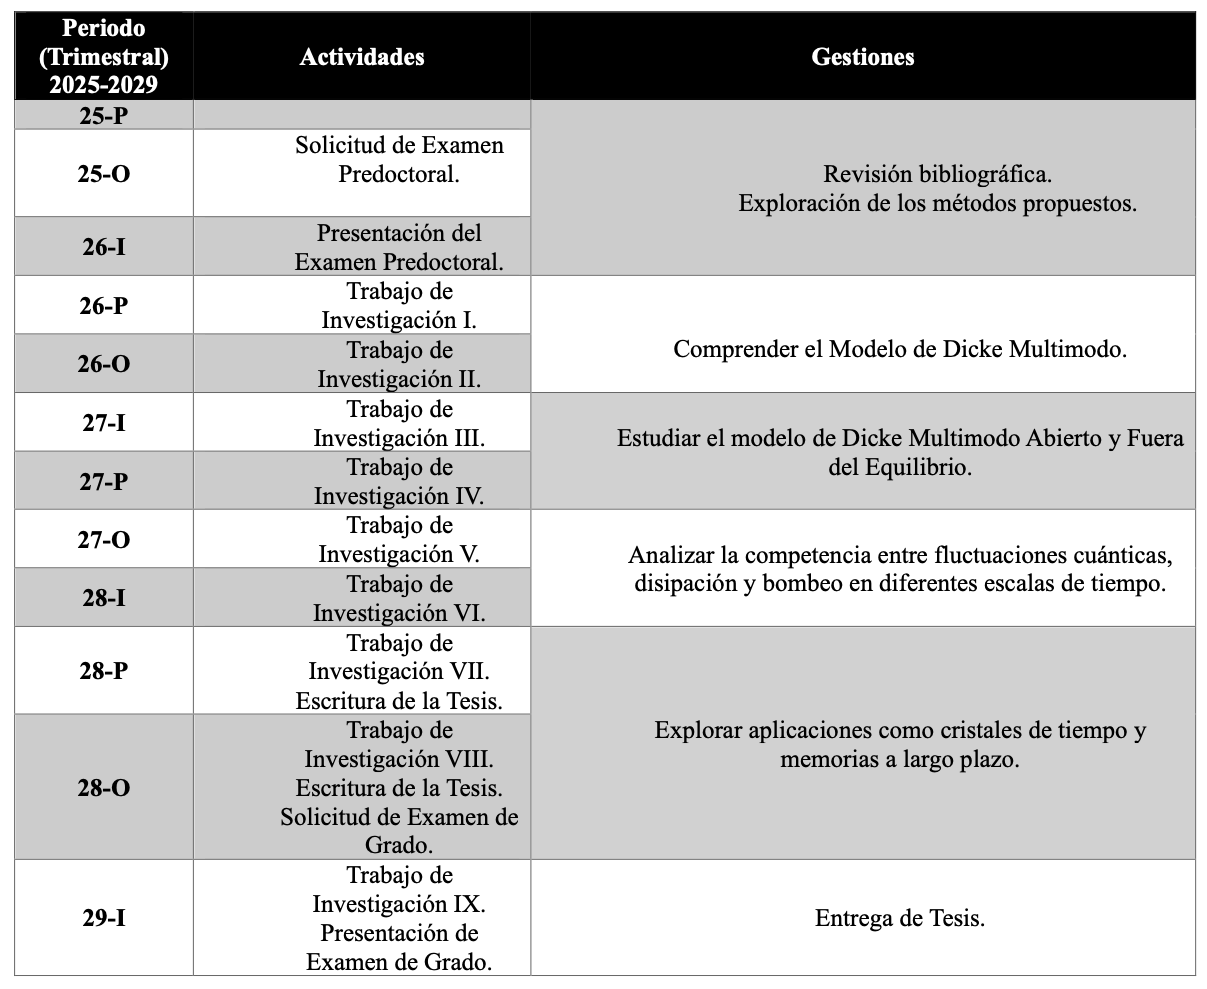
\includegraphics[width=1\linewidth]{Images/Tabla Cronologia.png}

\end{figure}

\begin{comment}
\noindent\textbf{Trimestre I-III}:
%%%
\begin{itemize}
    %%%
    \item  Extensión del Modelo de Dicke a sistemas multimodos. 
    %%%
    \begin{itemize}
        \item Estudiar el Modelo de Dicke, donde los átomos interactuan con múltiples modos fotónicos. 
        %%%
        \item Analizar las transiciones de fase superradiante y sus propiedades en sistemas multimodo. 
        %%%
    \end{itemize}
    %%%
    \item Efectos de desorden en el Modelo de Dicke. 
    %%%
    \begin{itemize}
        \item Investigar como el desorden en acoplamientos átomo-fotón afecta las transiciones de fase superradiantes. 
        %%% 
    \end{itemize}
\end{itemize}
%%%
\textbf{Trimestre IV-VI}:
%%%
\begin{itemize}
    %%%
    \item Extensión del Modelo de Dicke con disipación
    %%%
    \begin{itemize}
        \item Estudiar el modelo de Dicke en presencia de disipación utilizando la teoría de Keldysh. 
        %%%
        \item Analizar como la disipación afecta las transiciones de fase superradiantes y sus propiedades
        %%%
     \end{itemize}
    %%%
    \item  Dinámica de sistemas fuera de equilibrio en el Modelo de Dicke
    %%%
    \begin{itemize}
    %%%
        \item Utilizar el formalismo de Keldysh para estudiar la dinámica de relajación con desorden y disipación 
        %%%
        \item Explorar como las fluctuaciones cuánticas afecta la evolución temporal del sistema 
    \end{itemize}
\end{itemize}
%%%
\textbf{Trimestre VII-IX}:
\begin{itemize}
%%%
    \item Modelo de Dicke de dos fotones y Modelo de Rabi 
    %%%
    \begin{itemize}
    %%%
        \item Estudiar el Modelo de Dicke de dos fotones y Rabi en presencia de disipación. 
        %%%
        \item Analizar como la disipación afecta las transiciones de fase superradiantes y sus propiedades. 
    \end{itemize}
    %%%
    \item Teoría de renormalización funcional para sistemas abiertos.
    %%%
    \begin{itemize}
        \item Aplicar la teoría de renormalización funcional a sistemas abiertos. 
        %%%
        \item Estudiar como las fluctuaciones cuánticas y la disipación afectan las propiedades del sistema a diferentes escalas de energía. 
    \end{itemize}
\end{itemize}
%%%
\textbf{Trimestre X-XII}:
%%%
\begin{itemize} 
    %%%
    \item Aplicaciones en sistemas de Dicke fuera de equilibrio
    %%%
    \begin{itemize}
        \item Estudiar la posibilidad de cristales de tiempo en sistemas de Dicke acoplados a baños no markovianos. 
        %%%
        \item Explorar como la memoria a largo plazo afecta a la formación de estos estados. 
    \end{itemize}
\end{itemize}

\end{comment}







%%%%%%%%%%%%%%%%%%%%%%%%%%%%%%
%%%%%%%%%%%%%%%%%%%%%%%%%%%%%%
\section{Bibliografía}
\printbibliography[heading=none]
%%%%%%%%%%%%%%%%%%%%%%%%%%%%%%
%%%%%%%%%%%%%%%%%%%%%%%%%%%%%%

\end{document}
